\documentclass[aps,prb,reprint,noeprint,superscriptaddress]{revtex4-1}
\pdfoutput=1
\usepackage[utf8]{inputenc}
\usepackage[english]{babel}
\usepackage{microtype}
\usepackage{amsmath,amssymb,amsfonts}
\usepackage{braket}
\usepackage{bm}
\usepackage{graphicx}
\usepackage{booktabs}
\usepackage{comment}
\usepackage{siunitx}
\usepackage{float}
\usepackage[
    pdftitle={},
    pdfauthor={},
    colorlinks=true,
    unicode=true,
    pdfborder={0 0 0},
    allcolors=blue
]{hyperref}

\renewcommand{\vec}[1]{\bm{#1}}
\newcommand{\im}{\mathrm{i}}
\newcommand{\e}{\mathrm{e}}
\renewcommand{\Im}{\operatorname{\mathsf{Im}}}
\renewcommand{\Re}{\operatorname{\mathsf{Re}}}
\newcommand{\vk}{{\vec k}}
\newcommand{\vq}{{\vec q}}
\newcommand{\VV}[2]{\begin{pmatrix}#1\\#2\end{pmatrix}}
\newcommand{\VVT}[2]{\begin{pmatrix}#1 & #2\end{pmatrix}}
\newcommand{\VVV}[3]{\begin{pmatrix}#1\\#2\\#3\end{pmatrix}}
\newcommand{\VVVT}[3]{\begin{pmatrix}#1 & #2 & #3\end{pmatrix}}
\newcommand{\MM}[4]{\begin{pmatrix}#1 & #2 \\ #3 & #4\end{pmatrix}}

\begin{document}

\title{Time-resolved optical conductivity and Higgs oscillations\\in two-band dirty superconductors}

\author{Rafael Haenel}
\affiliation{Max Planck Institute for Solid State Research,
70569 Stuttgart, Germany}
\affiliation{Quantum Matter Institute, University of British Columbia, Vancouver V6T 1Z4, Canada}

\author{Paul Froese}
\affiliation{Max Planck Institute for Solid State Research,
70569 Stuttgart, Germany}
\affiliation{Quantum Matter Institute, University of British Columbia, Vancouver V6T 1Z4, Canada}


\author{Dirk Manske}
\affiliation{Max Planck Institute for Solid State Research,
70569 Stuttgart, Germany}

\author{Lukas Schwarz}
\affiliation{Max Planck Institute for Solid State Research,
70569 Stuttgart, Germany}


\date{\today}

%%%%%%%%%%%%%%%%%%%%%%%%%%%%%%%%%%%%%%%%%%%%%%%%%%%%%%%%
\begin{abstract}
...
\end{abstract}
%%%%%%%%%%%%%%%%%%%%%%%%%%%%%%%%%%%%%%%%%%%%%%%%%%%%%%%%




\maketitle


%%%%%%%%%%%%%%%%%%%%%%%%%%%%%%%%%%%%%%%%%%%%%%%%%%%%%%%%
\section{Introduction}
\label{sec:introduction}
%%%%%%%%%%%%%%%%%%%%%%%%%%%%%%%%%%%%%%%%%%%%%%%%%%%%%%%%

\begin{itemize}
	\item Ultrafast spectroscopy
	\item Collective modes in superconductors: Higgs, Goldstone (shifted to plasma energy due to Anderson-Higgs)
	\item In two-band superconductors: Additional out-of-phase Leggett mode, can couple to Higgs in nonequilibrium
	\item Difficulties excitation Higgs mode, in clean-limit only weak coupling
	\item In dirty superconductors: Coupling is enhanced. Activation of
		$\mathbf{p} \cdot \mathbf{A}$ term by momentum-converation
		braking impurity scattering.
	\item Discussion of Matthis Bardeen theory.
	\item This work: 1) Higgs oscillations in two-band sc. with bands in different limits, 2) Nonequilibrium optical conductivity, 3) Leggett mode in dirty-limit, 4) Prediction for MgB$_2$
\end{itemize}

This article is organized as follows. In Sec. \ref{sec:model} we briefly review
key aspects of the model as introduced by Murotani and Shimano []. We then
discuss the case of a single-band superconductor in a pump-probe scenario and
additionally with an assymetric supercurrent-inducing probe pulse in Sec.
\ref{sec:singleband}. We then extend these results to the two-band case in Sec.
\ref{sec:multiband} where we give explicit experimental predicitons for
pump-probe characterization of collective modes in MgB$_2$.







%%%%%%%%%%%%%%%%%%%%%%%%%%%%%%%%%%%%%%%%%%%%%%%%%%%%%%%%
\section{Model}
\label{sec:model}
%%%%%%%%%%%%%%%%%%%%%%%%%%%%%%%%%%%%%%%%%%%%%%%%%%%%%%%%

\begin{itemize}
	\item In this section show only the final formula, all derivation into the appendix A as the equations are similar to the Murotani paper.
	\item Show Hamiltonian, gap equation, Mattis-Bardeen replacement, general approach for calculating time evolution...
	\item I suggest putting the (final) equations for current, optical conductivity, $\delta\Delta(t)$ into the respective section, but in principle we could also put all equations in this section and show only the results in the following sections

	\item Used parameters (take general parameters for section III and IV where no Leggett mode occurs, Leggett mode is discussed later separately and MgB$_2$ will be also discussed later. Show the used parameters in these section)
	\item Implementation details? Are there any subtle points?
\end{itemize}


\begin{eqnarray}
	H_{\text{BCS}} = \sum_{i\mathbf{k}\sigma}  
	\varepsilon_{i\mathbf{k}}c_{i\mathbf{k}\sigma}^\dagger
	c_{i\mathbf{k}\sigma} + \sum_{i\mathbf{k}}^{}
	\left( \Delta_i c_{i\mathbf{-k}\uparrow }^\dagger
	c_{i\mathbf{k}\downarrow }^\dagger  \right) \,,
\end{eqnarray}

where $\varepsilon_{i\mathbf{k}} = s_i \left(\mathbf{k}^2/2m_i -
\varepsilon_{F_i}\right)$ and the superconducting order parameter is self-consistently determined by 
$\Delta_i = \sum_{j\mathbf{k}}^{}U_{ij} \langle c_{j-\mathbf{k}\downarrow
}c_{j\mathbf{k}\uparrow }\rangle$.

\begin{eqnarray*}
	H_{\text{p-p}} = -\sum_{i\mathbf{kk'}\sigma}^{}
	\mathbf{J}_{i\mathbf{kk'}} \cdot \mathbf{A} \,
	c_{i\mathbf{k}\sigma}^\dagger  c_{i\mathbf{k}'\sigma} +
	\sum_{i\mathbf{k}\sigma}^{} \frac{s_i e^2}{2m_i} \mathbf{A}^2 \,
	c_{i\mathbf{k}\sigma}^\dagger c_{i\mathbf{k}\sigma}
\end{eqnarray*}

\begin{eqnarray*}
	\langle \left|\mathbf{e} \cdot
	\mathbf{J}_{i\mathbf{kk'}}\right|^2\rangle_{\text{Av}}
	&=& \int \frac{d\Omega_\mathbf{k}}{4\pi} \frac{d\Omega_\mathbf{k}'}{4\pi}
	\left|\mathbf{e} \cdot \mathbf{J}_{i\mathbf{kk'}}\right|^2
	\\
	&\approx& \frac{(e v_{F_i})^2}{3 \pi N_i(0)} 
	\frac{\gamma_i}{(\varepsilon-\varepsilon')^2 + \gamma_i^2}
\end{eqnarray*}

Discussion of $A, A^2$.

The full Hamiltonian is given by $H = H_{BCS} + H_{p-p}$.







Shortcoming of the model. Momentum-angle averaging removes information about
polarization, momentum of photon. The gap oscillates with its equilibrium value
and not $\Delta_{\infty}$. Also, the results are an expansion in $A$ up to third
order. Specifically, the gap in only included up to second order (the only
nonzero term) which makes it hard to say when this approximation becomes
invalid. The dependence of the gap on fluence is linear up to this order.


\section{Single-band superconductivity}
\label{sec:singleband}

Motivated by the experiment of Matsunaga et al. [] we choose parameters
$\Delta_{\text{eq}}=\SI{1.3}{\milli\electronvolt}$,
$\varepsilon_{F}=\SI{1}{\electronvolt}$, $m=0.78 m_e$, $s=1$ that reflect
measurements and ab-initio calculations on NbN [DFT-reference].
The Debye energy for NbN is order order of $\omega_D = \SI{5}{\milli\electronvolt}$, but
for better numerical resolvability we choose $\omega_D =
\SI{2}{\milli\electronvolt}$.

A characteristic property of a pump pulse is its pulse length $\tau$ in units of the natural
timescale of the superconductor, $\hbar/\Delta$. For $\tau \ll \hbar / \Delta$
the superconductor is \textit{quenched}, while it is adiabatically driven in the
opposite limit of $\tau \gg  \hbar / \Delta$. Here, we investigate a quench
scenario with $\hbar\tau/\Delta=x$ by fitting the pulse form $A(t) = A_0 \exp\left( -(t-t')^2/2\tau^2
\right)\cos \Omega t$ to the reported data of [Matsunaga]. The resulting
electrical field waveform is shown in panel A of Fig. \ref{fig:singleband-gap}. 


\begin{figure}[ht]
	\centering
	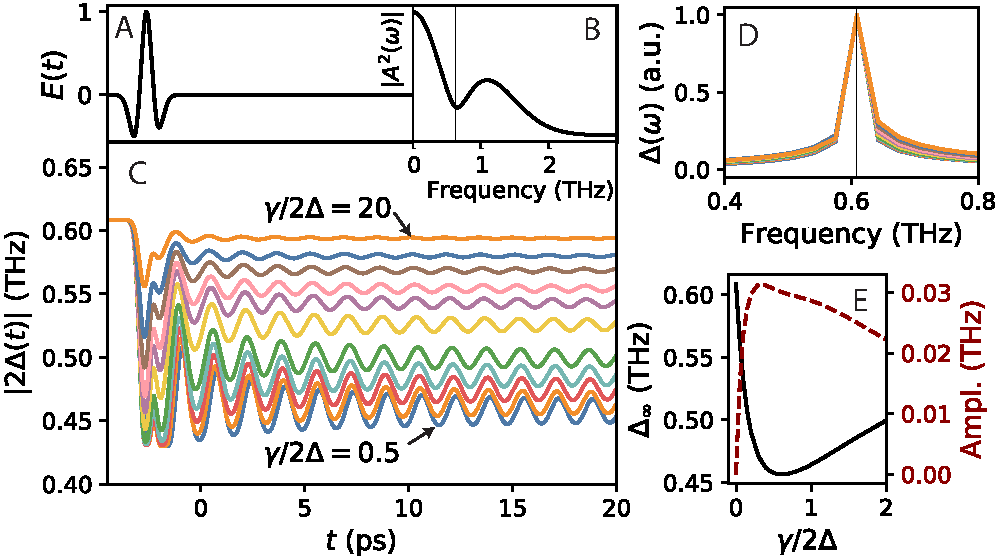
\includegraphics[width=\columnwidth]{figures/fig1.pdf}
	\caption{(A) Pulse field $E(t)$ realizing a qunech. (B) Spectral
	composition $|A(\omega)|$. The gray shaded area illustrates the
quasi-particle continuum. (C) Spectral compositon $A^2(\omega)$ of the second
order component $A^2(t)$ responsible for excitation of collective modes. The
peak around zero frequency corresponds to a DFG process while the peak at finite
$\SI{1.2}{\tera\hertz}$ is a SFC process. (C) Evolution of the magnitude of the
order parameter $\left|2\Delta(t)\right|$ for impuritiy strength varying from
$\gamma/2\Delta=0.5$ to $20$ and Fourier spectrum of the gap oscillations (D).
(E) Relaxation value $\Delta_{\infty}$ and amplitude of oscillation show a very
similar dependence as a function of disorder strength which has maximum effect
at around $\gamma \approx \Delta$.}

$\Delta_{\infty}$ is given by the overlap of the pulse with the density of
states of the quasiparticel continuum, 
$$\Delta_{\infty} \propto
\int_{}^{}d\omega N(\omega) A(\omega) \approx N(\varepsilon_F)
\int_{\varepsilon_F}^{\infty}d\omega A(\omega)$$.
\label{fig:singleband-gap}
\end{figure}

\begin{figure}[ht]
	\centering
	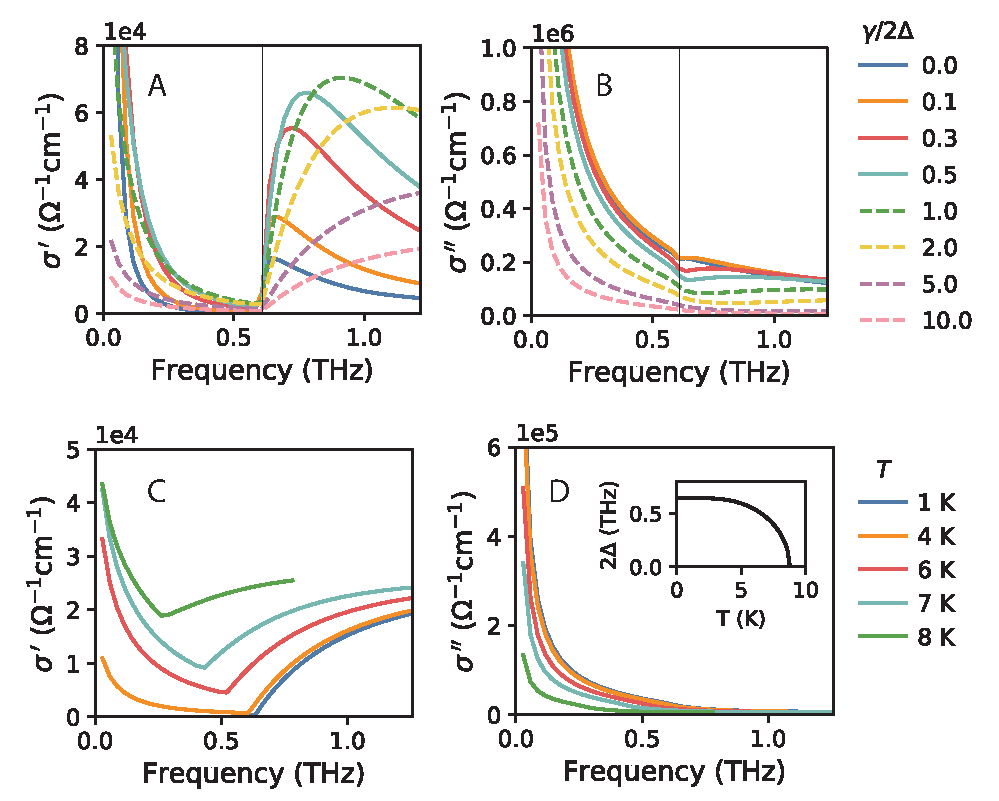
\includegraphics[width=\columnwidth]{figures/fig2.pdf}
	\caption{Real part $\sigma'$ (A,C) and imaginary part $\sigma''$ (B,D)
		of optical conductivities to first order in $A$ 
	for various impurity scattering rates at $T=\SI{4}{\kelvin}$ (A,B) and
various temperatures at $\gamma/2\Delta=10$. $\sigma'$ show a characteristic
conductivity gap below $T_C$ and both $\sigma'$, $\sigma''$ diverge in the
static limit.}
\end{figure}

\begin{figure}[ht]
	\centering
	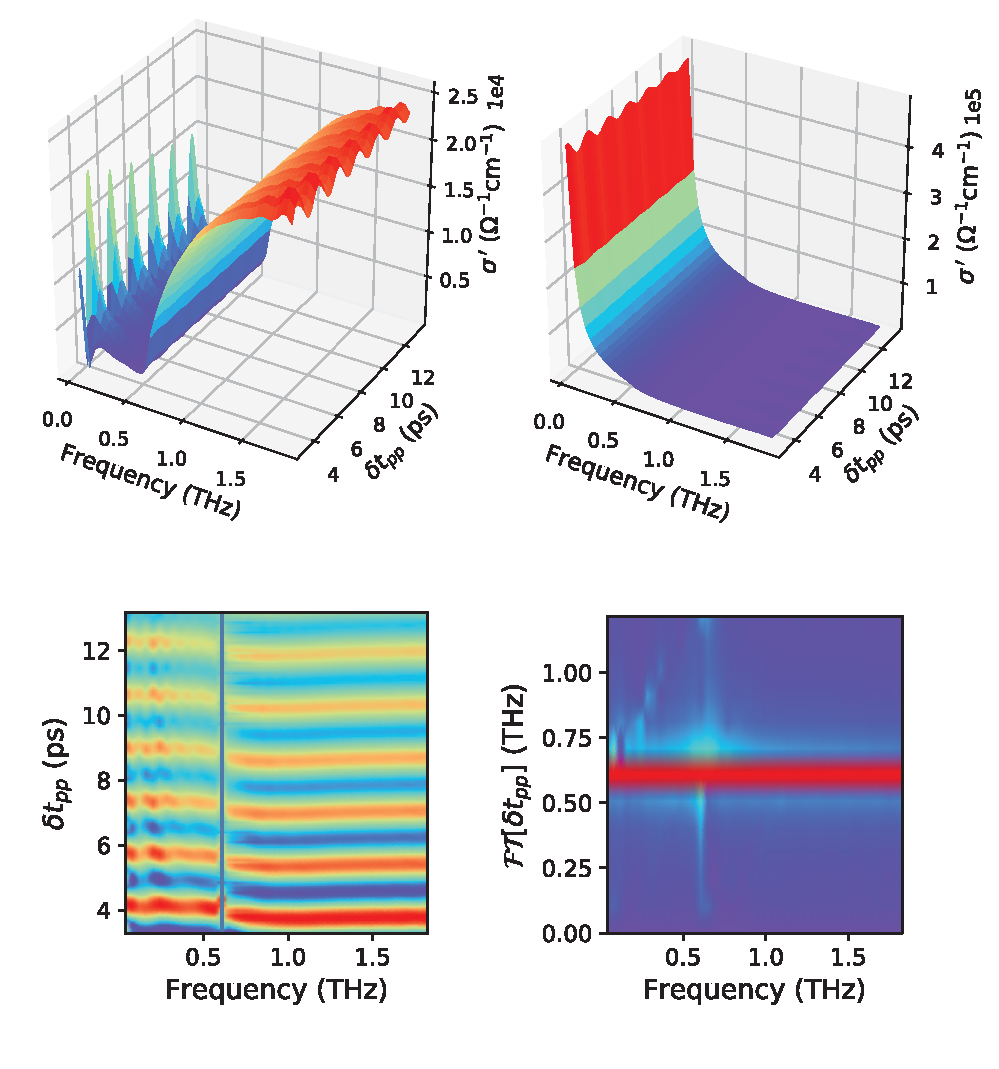
\includegraphics[width=\columnwidth]{figures/fig3.pdf}
	\caption{(A,B) Conductivity spectra for sweeped pump-probe delay $\delta
	t_{\text{p-p}}$ to third order in $A$. (C) False-color plot of
$\sigma' $ which was average-subtracted and normalized to show the oscillations.
A phase shift occurs across the resonance at $2\Delta_{\text{eq}}$ of the quench pulse
frequency. (D) Fourier spectrum of panel (C) showing that frequency of
conductivity oscillation is peaked at $2\Delta_{\text{eq}}$.}
\end{figure}
%\begin{comment}
\section{Multi-band superconductivity}
\label{sec:multiband}

\begin{figure}[ht]
	\centering
	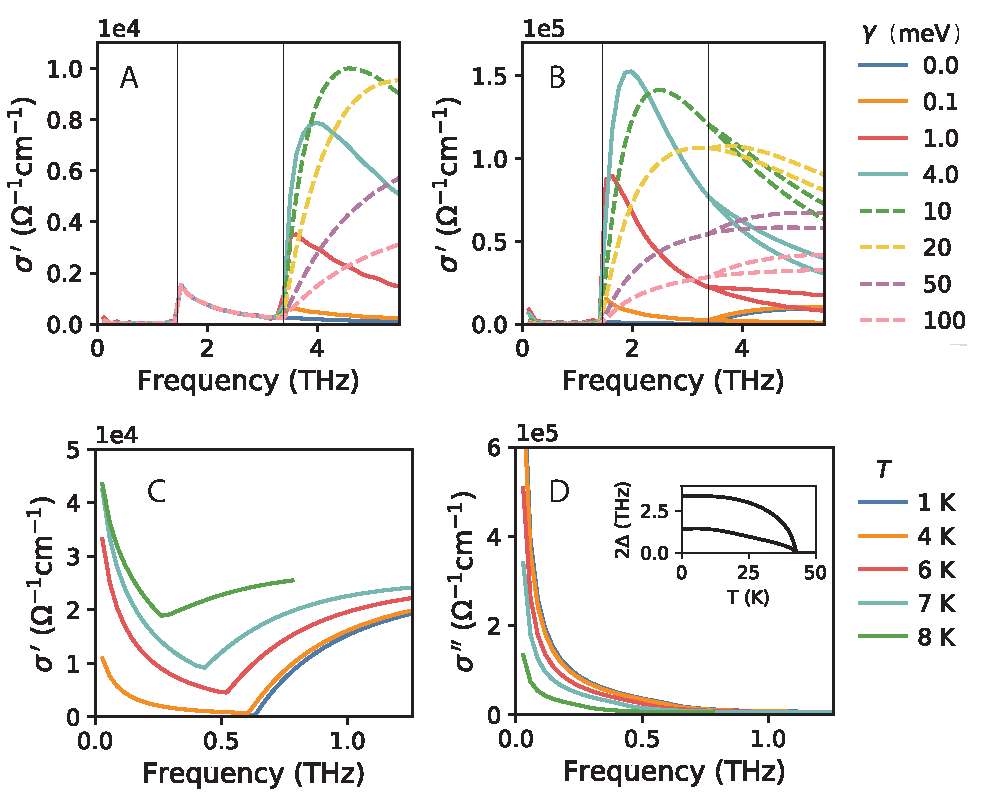
\includegraphics[width=\columnwidth]{figures/m-fig1.pdf}

	\caption{Real part $\sigma'$ (A,C) and imaginary part $\sigma''$ (B,D)
		of optical conductivities to first order in $A$ 
	for various impurity scattering rates at $T=\SI{4}{\kelvin}$ (A,B) and
various temperatures at $\gamma/2\Delta=10$. $\sigma'$ show a characteristic
conductivity gap below $T_C$ and both $\sigma'$, $\sigma''$ diverge in the
static limit.}
	
$\Delta_{\infty}$ is given by the overlap of the pulse with the density of
states of the quasiparticel continuum, 
$$\Delta_{\infty} \propto
\int_{}^{}d\omega N(\omega) A(\omega) \approx N(\varepsilon_F)
\int_{\varepsilon_F}^{\infty}d\omega A(\omega)$$.
\label{fig:singleband-gap}
\end{figure}

%%%%%%%%%%%%%%%%%%%%%%%%%%%%%%%%%%%%%%%%%%%%%%%%%%%%%%%%
\section{Higgs oscillations}
\label{sec:higgs_oscillations}
%%%%%%%%%%%%%%%%%%%%%%%%%%%%%%%%%%%%%%%%%%%%%%%%%%%%%%%%

\begin{itemize}
	\item Equation for Current
	\item Equation for optical conductivity
	\item Present and discuss equilibrium optical conductivity in Fig. 1 for the four different limit cases, used in the rest of the paper
\end{itemize}


\begin{figure}[H]
    \centering
    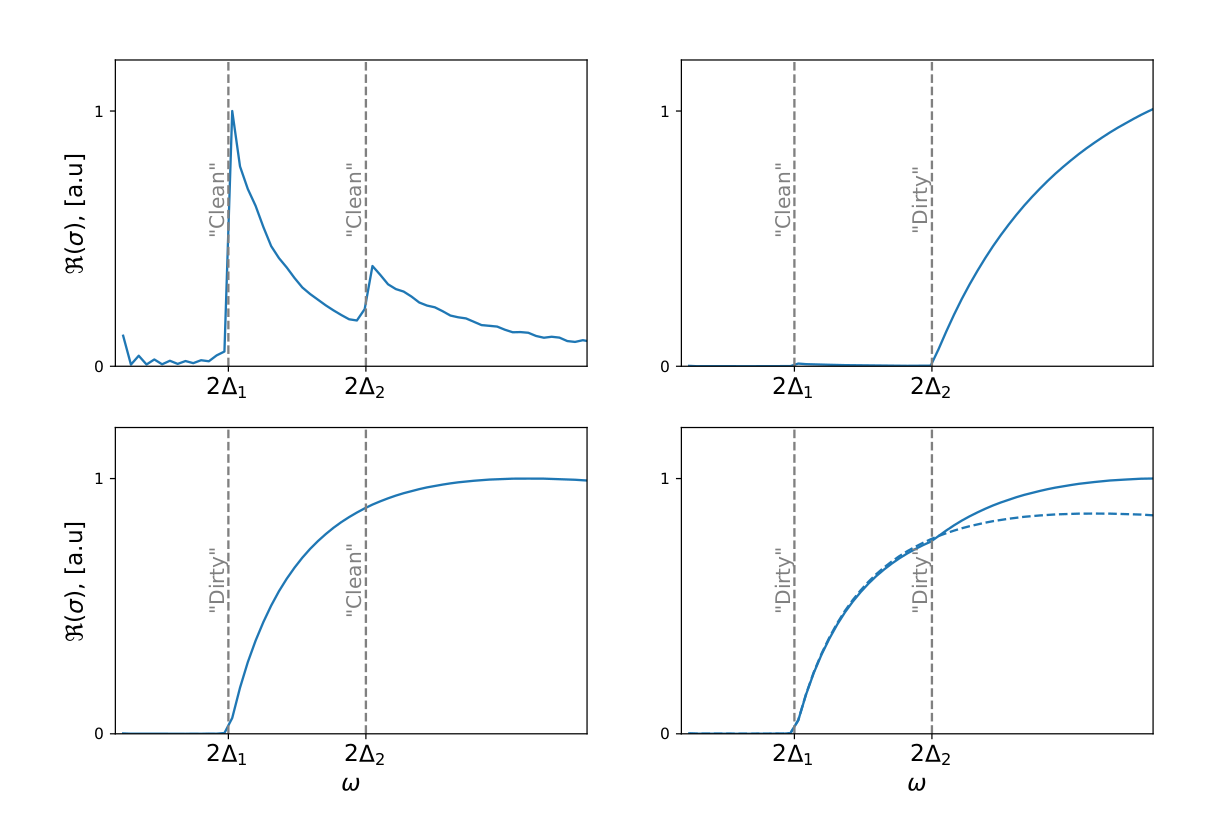
\includegraphics[width=\columnwidth]{figures/two_band_cond.png}
    \caption{\label{fig:two_band_cond}%
    Equilibrium optical conductivity of a two-band superconductor with gaps in different impurity scattering limits (clean-clean case rescaled as response is much smaller?)}
\end{figure}%

\begin{itemize}
	\item Equation for $\delta\Delta(t)$
	\item Show and discuss Higgs oscillations in Fig. 2 of the four cases with a suitable pump pulse (refer to appendix B for details about the pump pulse)
\end{itemize}

\begin{figure}[H]
    \centering
    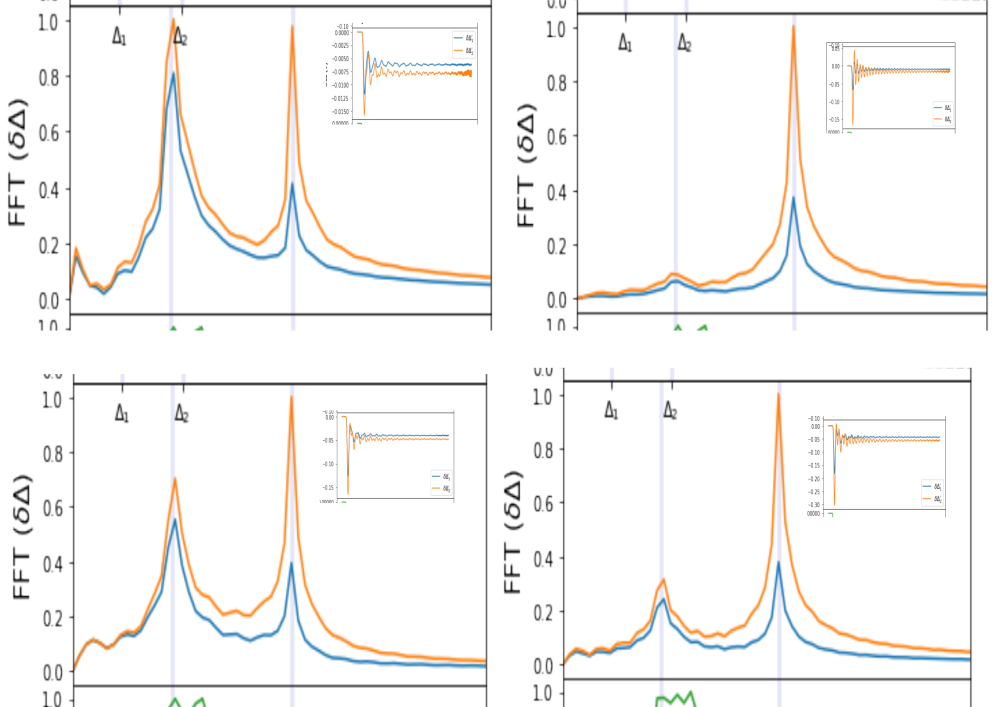
\includegraphics[width=\columnwidth]{figures/gap_osci.png}
    \caption{\label{fig:gap_osci}%
    Higgs oscillations excited by a pump pulse with enough bandwidth to cover both gaps for the different impurity scattering limits shown in Fig.~\ref{fig:two_band_cond}}
\end{figure}%








%%%%%%%%%%%%%%%%%%%%%%%%%%%%%%%%%%%%%%%%%%%%%%%%%%%%%%%%
\section{Nonequilibrium optical conductivity}
\label{sec:noneq_cond}
%%%%%%%%%%%%%%%%%%%%%%%%%%%%%%%%%%%%%%%%%%%%%%%%%%%%%%%%

\begin{itemize}
	\item Equation for nonequilibrium optical conductivity with two pulses. Maybe here more details (instead of appendix), as this is not covered by the Murotani paper
	\item Show and discuss nonequlibrium conductivity in Fig. 3.
	\item More figures of nonequilibrium conductivity? Suggestions: Imaginary part, maybe appendix. Nice 3d plot. Oscillations along cuts.
\end{itemize}


\begin{figure}[H]
    \centering
    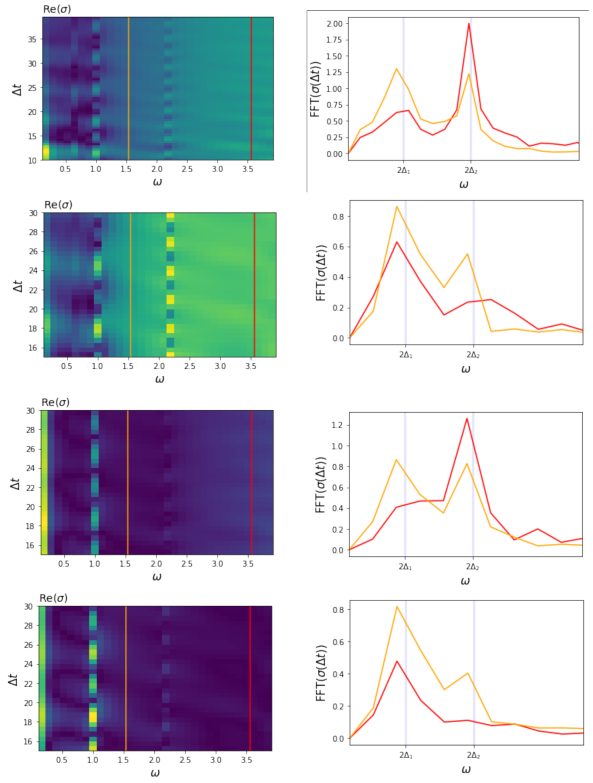
\includegraphics[width=\columnwidth]{figures/noneq_cond.png}
    \caption{\label{fig:noneq_cond}%
    Nonequilibrium optical conductivity of a pump-probe experiment for the different impurity scattering limits shown in Fig.~\ref{fig:two_band_cond}}
\end{figure}%


%%%%%%%%%%%%%%%%%%%%%%%%%%%%%%%%%%%%%%%%%%%%%%%%%%%%%%%%
\section{Leggett mode}
\label{sec:leggett_mode}
%%%%%%%%%%%%%%%%%%%%%%%%%%%%%%%%%%%%%%%%%%%%%%%%%%%%%%%%

\begin{itemize}
	\item Definition, equation of Leggett mode
	\item Parameters for Fig.4 where Leggett mode occurs
	\item Discuss Fig. 4
	\item Maybe rethink what exactly to show in Fig. 4
	\item New plot of time-resolved conductivity showing Leggett mode?
\end{itemize}

\begin{figure}[H]
    \centering
    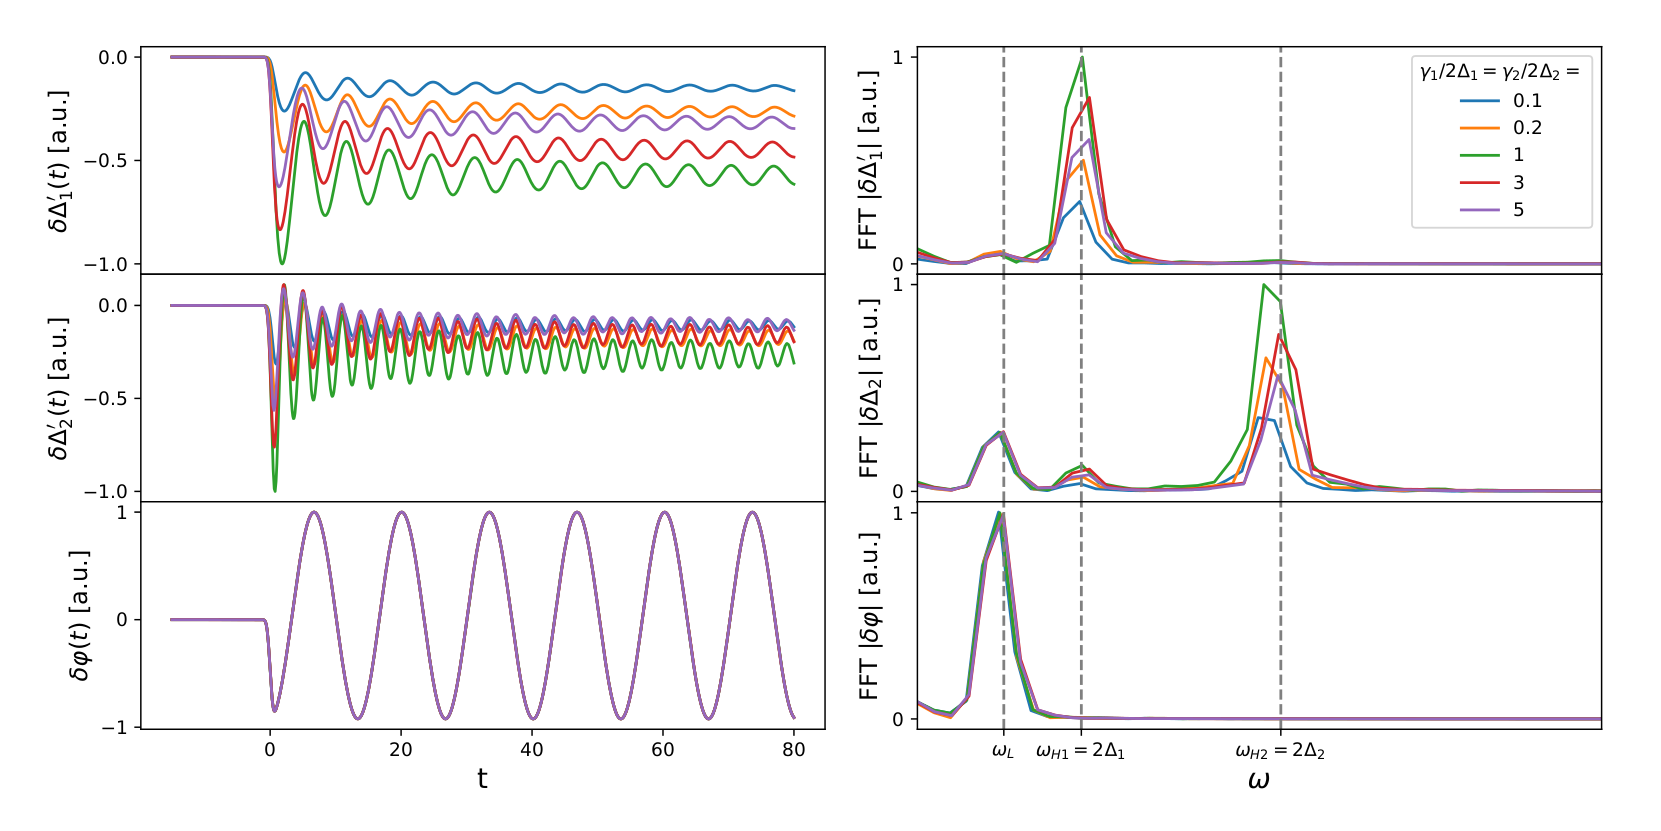
\includegraphics[width=\columnwidth]{figures/leggett_oscillations.png}
    \caption{\label{fig:leggett_oscillations}%
    Induced amplitude (Higgs) and out-of-phase (Leggett) oscillations of a two-band superconductor for different impurity scattering rates}
\end{figure}%

\begin{itemize}
	\item Discuss Fig. 5 for varying coupling strength and compare with clean limit result
\end{itemize}

Leggett mode has been potentially measured in between the two gaps. Discuss this
and also refer to Schnyder Nature Comm. Figure out the parameter regime that
inverted the gaps. Reproduce (or see what was wrong) with Murotani who also
choose parameters such that the Leggett mode is inside the gap.

\begin{figure}[H]
    \centering
    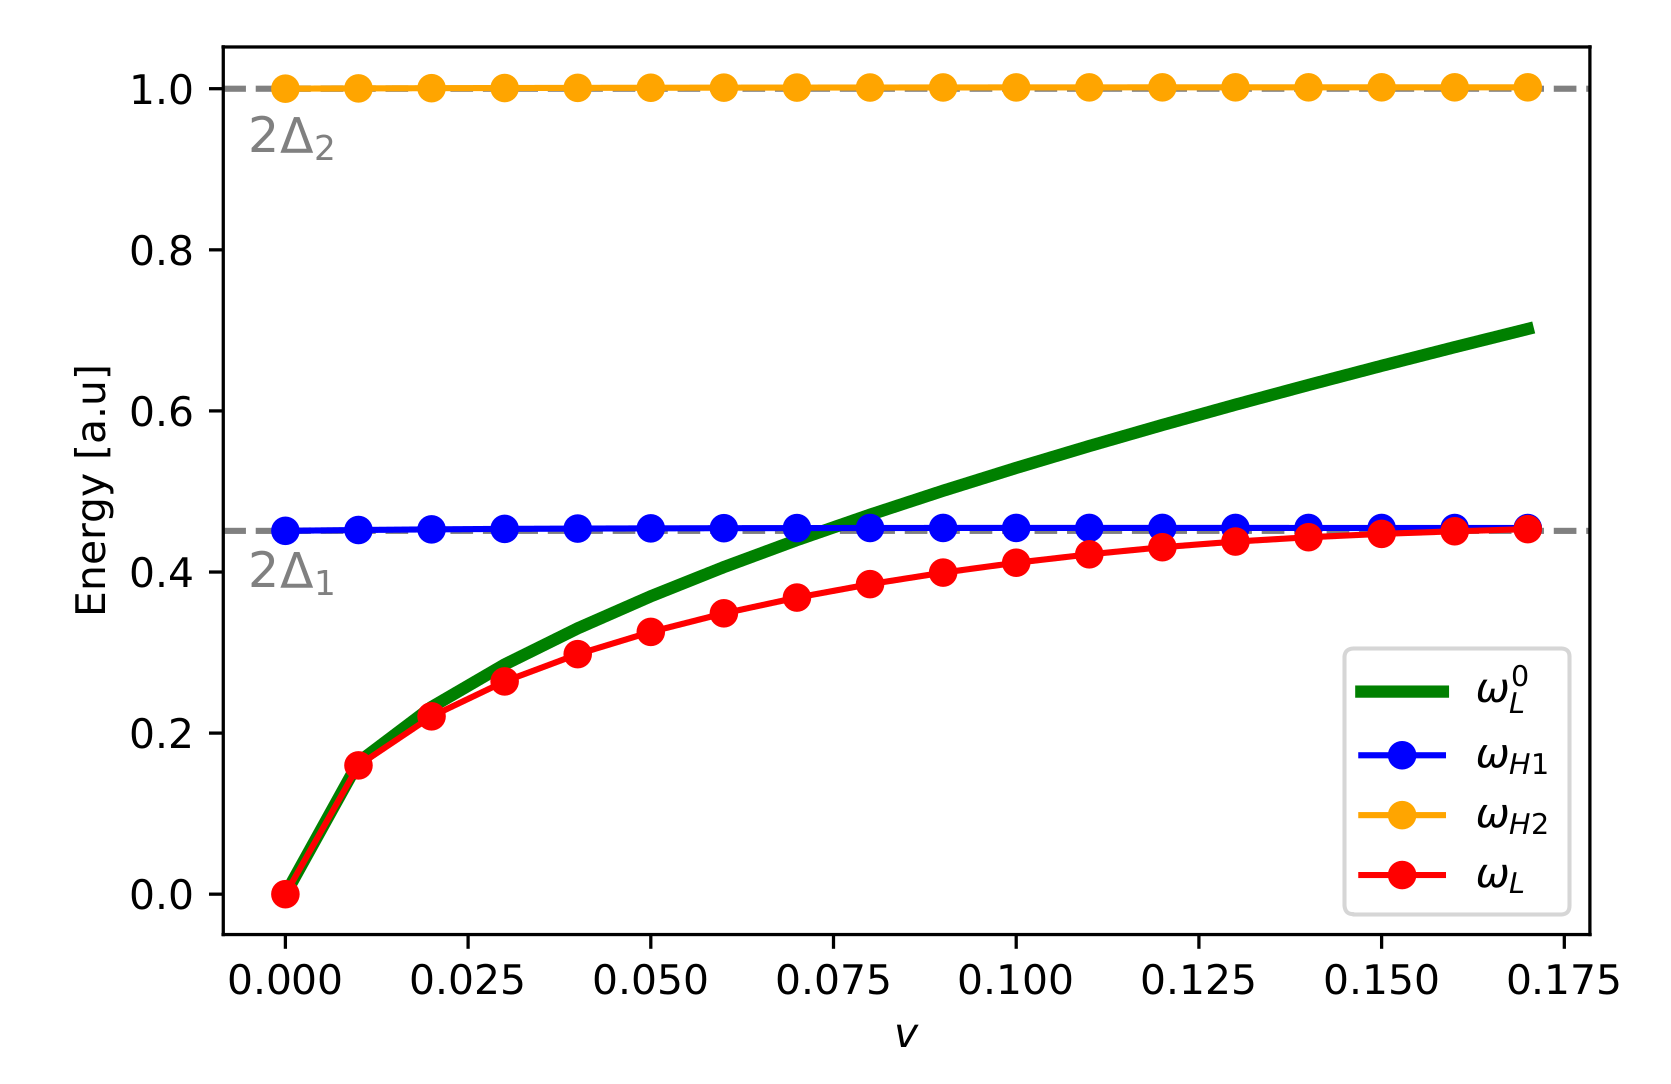
\includegraphics[width=\columnwidth]{figures/leggett_coupling.png}
    \caption{\label{fig:leggett_coupling}%
    Frequency of Leggett mode as function of interband coupling strength in the dirty limit}
\end{figure}%



%%%%%%%%%%%%%%%%%%%%%%%%%%%%%%%%%%%%%%%%%%%%%%%%%%%%%%%%
\section{MgB$_2$}
\label{sec:mgb2}
%%%%%%%%%%%%%%%%%%%%%%%%%%%%%%%%%%%%%%%%%%%%%%%%%%%%%%%%

\begin{itemize}
	\item Parameters which match MgB$_s$
	\item Show prediction in Fig. 6 of equilibrium conductivity, Higgs oscillations, nonequilibrium conductivity
\end{itemize}

\begin{figure}[H]
    \centering
    %\includegraphics[width=\columnwidth]{figures/mgb2.png}
    \Huge{TODO}
    \caption{\label{fig:mgb2}%
    Result with parameters for MgB$_2$ a) Equilibrium optical conductivity, b) Higgs oscillations, c) pump-probe conductivity and spectra}
\end{figure}%



%%%%%%%%%%%%%%%%%%%%%%%%%%%%%%%%%%%%%%%%%%%%%%%%%%%%%%%%
\section{Conclusion}
\label{sec:conclusion}
%%%%%%%%%%%%%%%%%%%%%%%%%%%%%%%%%%%%%%%%%%%%%%%%%%%%%%%%

...







%%%%%%%%%%%%%%%%%%%%%%%%%%%%%%%%%%%%%%%%%%%%%%%%%%%%%%%%
\begin{acknowledgments}
...
\end{acknowledgments}
%%%%%%%%%%%%%%%%%%%%%%%%%%%%%%%%%%%%%%%%%%%%%%%%%%%%%%%%






%%%%%%%%%%%%%%%%%%%%%%%%%%%%%%%%%%%%%%%%%%%%%%%%%%%%%%%%
\bibliography{literature}
%%%%%%%%%%%%%%%%%%%%%%%%%%%%%%%%%%%%%%%%%%%%%%%%%%%%%%%%




%%%%%%%%%%%%%%%%%%%%%%%%%%%%%%%%%%%%%%%%%%%%%%%%%%%%%%%%
%\end{comment}
\appendix
%%%%%%%%%%%%%%%%%%%%%%%%%%%%%%%%%%%%%%%%%%%%%%%%%%%%%%%%


%%%%%%%%%%%%%%%%%%%%%%%%%%%%%%%%%%%%%%%%%%%%%%%%%%%%%%%%
\section{Derivation of nonequilibrium optical conductivity}
\label{sec:derivation_noneq_cond}
%%%%%%%%%%%%%%%%%%%%%%%%%%%%%%%%%%%%%%%%%%%%%%%%%%%%%%%%


\begin{itemize}
	\item Put here all equations and derivations of the main results
\end{itemize}






%%%%%%%%%%%%%%%%%%%%%%%%%%%%%%%%%%%%%%%%%%%%%%%%%%%%%%%%
\section{Influence of pump pulse frequency}
\label{sec:influence_pump_pulse_freq}
%%%%%%%%%%%%%%%%%%%%%%%%%%%%%%%%%%%%%%%%%%%%%%%%%%%%%%%%

\begin{itemize}
	\item Discuss influence of pump pulse frequency and bandwith to excite only one or both Higgs mode
	\item Show result in Fig. 7
\end{itemize}

\begin{figure}[H]
    \centering
    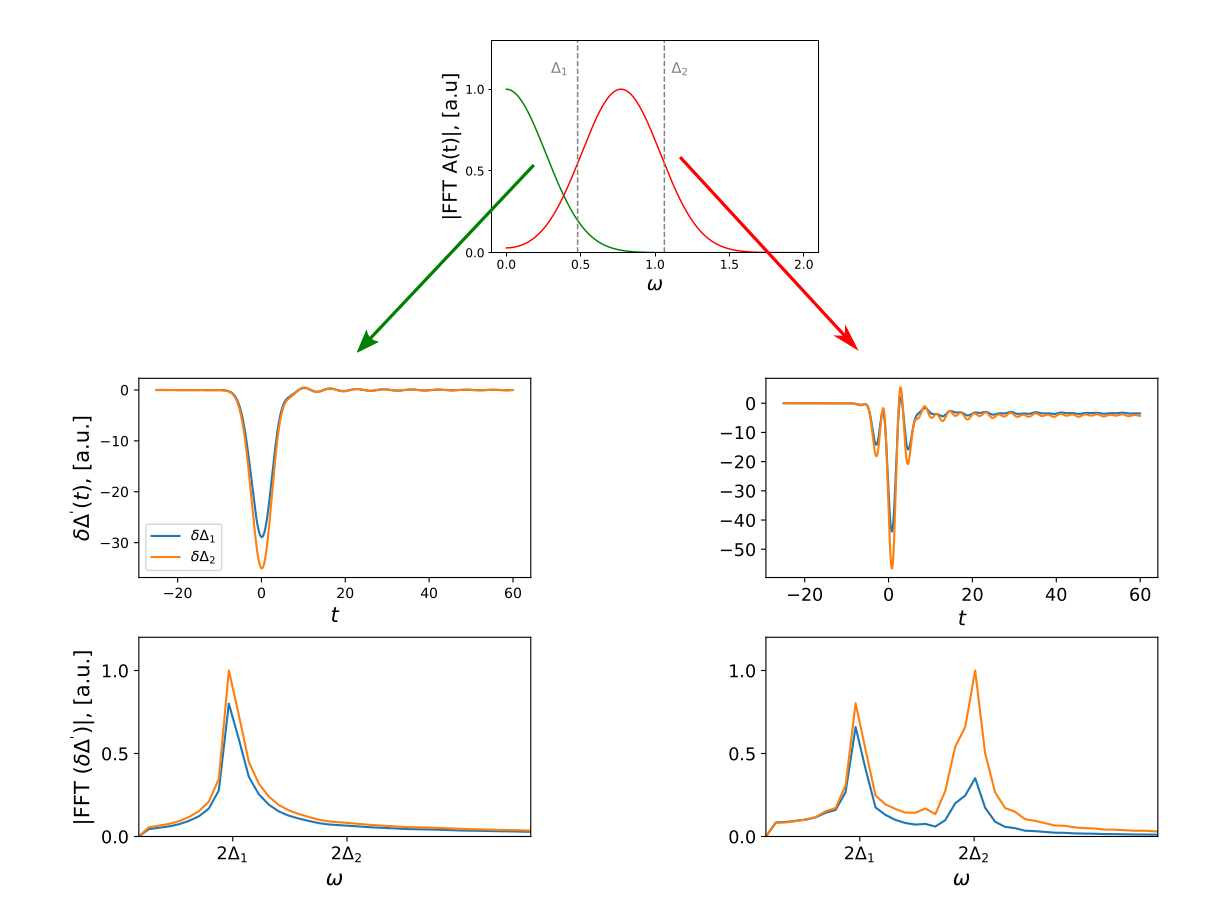
\includegraphics[width=\columnwidth]{figures/influence_pump_pulse_freq.png}
    \caption{\label{fig:influence_pump_pulse_freq}%
    Influence of pump pulse frequency}
\end{figure}%



\end{document}
